\section{Case Study: \appname}
\label{sec:formal}

\chiao{<= 3 pages}

In this section, we present the formal definition of \appname problem.
Then we develop a state machine model executing in the physical environment,
and finally, using this model we show that it meets the key requirements of the problem.
One of the outcomes of this analysis is the identification of a list of precise assumptions of sensors,
quantization, and \sayan{fill in}, that need to be checked separately for obtaining end-to-end, system-level guaranteed.

%\section{Koord Software Stack}
\label{sec:software}

\subsection{Runtime system}



To run a $\lgname$ program (hardware or simulation), the user has to provide a configuration file, with
\begin{inparaenum}
    \item the number of agents,
    \item in case of simulation, the initial positions of the agents and the length of the simulation and
    \item in case of hardware deployment their IP addresses,
    and the localization system.
\end{inparaenum}

\subsection{Key environment assumptions}


\subsubsection{Periodic event execution semantics}


\subsubsection{Shared variable implementation over message passing}


\subsubsection{Known set of participants}
\subsubsection{Portability and heterogeneity}


\subsection{Simulator}
\subsubsection{gazebo environment}
\subsubsection{car model}
\subsubsection{lidar}
\subsubsection{positioning}
\subsubsection{sampled sensing}
\subsubsection{synchronization issues}

\subsection{The Distributed Mapping Problem}
In this section, we introduce the distributed mapping problem. Informally, the problem requires a set of robots to collaboratively mark the position of static \emph{obstacles} within a given area $D$, which any robot should avoid while moving in $D$.The key difference between distributed SLAM and this application is that we assume that the robots know their \emph{global coordinates} within the area of deployment. They are only attempting to map the static obstacles within this area. We currently assume that the only sensors available for sensing obstacles are LIDAR based, and the robots are constrained to move in a 2-D space.


\subsubsection{Preliminaries}
\label{sec:prelims}
We first set up the terminology and assumptions to discuss our approach to this problem.

The mapping problem is defined over a (\emph{bounded}) domain $D$, a bounded rectangle in $\mathbb{R}^2$ given by $[a_1,a_2]\times [b_1,b_2]$.

\begin{definition}
    A \emph{quantization} of a bounded domain $D$ is defined as a mapping $\qfunc:D \mapsto \qdom$ where $\qdom = \left\{q_{ij}\right\}_{i\in [1..n_x], j\in [1..n_y]}$ such that every $q_{ij}$ corresponds to a \emph{grid rectangle} $[x_i, x_{i+1}] \times [y_j, y_{j+1}]$.
\end{definition}

We assume the existence of a \emph{ground truth} function $\world : D\mapsto \left\{0,1\right\}$, where $\forall \Vec{x} \in D$, $$\world(\Vec{x}) = \begin{cases}
                                                                                                                                                                        1\ \mbox{if there is an obstacle at }\Vec{x}\\
                                                                                                                                                                        0\ \mbox{otherwise}
\end{cases}
$$


\begin{definition}
    Given a quantized domain $Q$, a \emph{\qdfunc} over $Q$ is any function $F$ with the signature $Q^\prime \mapsto \left\{0,1\right\}$, where $F$ is only defined on $Q^\prime \subset Q$, and it maps each $q_i \in Q^\prime$ to either 0 or 1.
\end{definition}


Given any quantization $Q$ of the domain $D$ given by $\qfunc:D\mapsto Q$, the corresponding \qdfunc
$\world_Q : Q \mapsto \left\{0,1\right\}$ is defined as follows,  $$\world_Q(q) = \begin{cases}
                                                                                      1\ \Leftrightarrow \exists \Vec{x}\in D, \qfunc(\Vec{x}) = q \wedge \world(\Vec{x}) = 1 \\
                                                                                      0\ \mbox{otherwise}
\end{cases}
$$


\rg{Consider that there is a set of ground robots $[N]$, which are tasked with creating a mapping of static obstacles in $Q$ collaboratively by constructing local mappings based on sensed information.}


\begin{definition}
    The \emph{sensing area} of a robot $i$ at position $\pos(i)\in D$ is defined by $\sensarea_i: Q \mapsto 2^{Q}$, such that there is a \qdfunc\ $\rmap : \sensarea_i \mapsto \left\{0,1\right\}$, where $$\forall q \in \sensarea_i(\qfunc(\pos_i)), \rmap(q) = \world_Q(q).$$
    Given a robot $i \in [N]$, $\sensarea_i$ may depend both on the position of the robot as well as the range of the LIDAR scanner.
\end{definition}



Let $\map_i:Q\mapsto \left\{-1,0\right\}$ denote a \qdfunc \emph{local} to robot $i$, which we see as a \emph{software state} for a given robot $i$.  % $\map_i(q) = 1$ indicates that according to robot $i$, there is an obstacle in $q$, $\map_i(q) = 0$ indicates that according to robot $i$, $q$ is unoccupied, and $\map_i(q) = -1$ indicates that robot $i$ doesn't have information about $q$.



We assume that given $\Vec{x} \in q, \forall \Vec{x^\prime} \in q, \sensarea(\Vec{x}) \subseteq \sensarea(\Vec{x^\prime})$. We can now state the 2-d distributed mapping problem, $\mapprob$ as follows. \begin{quote}
{\em Given a quantization, $\qfunc:D\mapsto Q$ of a 2-d domain $D\subset \mathbb{R}^2$, a ground truth function $\world:D \mapsto \left\{0,1\right\}$, a set of robots $[N]$ , for each robot $i \in [N]$ construct an \emph{occupancy map} which is a \qdfunc, $\map_i: Q_i \mapsto \left\{1,0\right\}$, $Q_i\subseteq Q$.
}
\end{quote}

% \rg{We can \emph{combine} the elements of the set of \emph{local maps}, $\{\map_i\}_{i\in [N]}$ to form a \emph{global} occupancy mapping. }

Having stated the problem, we now define the notion of soundness of a proposed occupancy map.
\begin{definition}
    \label{soundness}
    For a robot $i$, a proposed occupancy mapping over $Q_i\subset Q$, given by $\map_i: Q_i \mapsto \left\{-1,0\right\}$ is \emph{sound} if :
    \begin{itemize}
        \item $\map_i(q) = v \Rightarrow \world_Q(q)  = v$
        \item $\forall v \in \left\{0,1\right\}\world_Q(q) = v \Rightarrow \map(q) = v \vee q\notin Q_i$
    \end{itemize}
\end{definition}


These two statements collectively state that given a proposed occupancy map, \emph{any grid rectangle in the domain of the occupancy map marked as 0 is indeed obstacle free, and if it is marked as 1 then there is indeed an obstacle at least partially in it.}

A vacuously correct (sound) solution to $\mapprob$ given $D, \qfunc$ and $\world_Q$ is $\forall i \in [N]$, $$\map_i : Q_i \mapsto \left\{0,1\right\}, Q_i = \phi$$ To allow for more interesting solutions than the one stated above, we assume that we are given that initially, each robot $i\in[N]$ starts at a grid rectangle with no obstacle, the sensed area of each robot $i$ is non empty, and there is at least one obstacle free rectangle within the sensed area of each robot:
$\forall i \in [N], \world_Q(q^0_i) = 0 \wedge \exists q \in \sensarea(q^0_i), \world_Q(q) = 0 $ and
where $q^0_i = \qfunc(\pos_0(i))$, and $\pos_0(i)$ denotes the initial position of robot $i$.


\begin{definition}
    Given  $i , j \in [N]$, two proposed occupancy mappings $\map_i: Q_i\mapsto\left\{0,1\right\}$ and $\map_j: Q_j\mapsto \left\{0,1\right\}$, are consistent only if $\forall q \in Q_i \cup Q_j, \map_i(q) = \map_j(q)$.
\end{definition}

    Given $\map_i$, $\map_j$, and $q\in Q_i \cup Q_j$ , let $\map_i(q) = 1$, and $\map_j(q) = 0$. Suppose $\map_i$ is sound, then $\world_Q(q) = 1$, which implies $\map_j$ is not sound. By the same argument, if $\map_j$ is sound, $\map_i$ is not. A set of proposed mappings $\left\{\map_i\right\}_{i\in [N]}$ can only be sound if they are pairwise consistent.

%We assume that if robot $i$ is at position $\pos(i)$, and it detects an obstacle in $q \in \sensarea(\qfunc(\pos(i)))$, then $q$ does contain an obstacle, otherwise it does not. The point of this presentation isn't dealing with the issue of potentially false positives while identifying an obstacle. A robot partially constructs a grid occupancy function by assigning values to the grid rectangles in its \emph{sensed} area.


%\begin{lemma}
%    \label{ext}
%    Suppose robot $i$ is at $\pos(i)\in D$, and $\exists(q^\prime)\in \sensarea(\pos(i))$,
%    s.t $\map_i(q) = -1$. Consider a mapping, $\map^\prime_i:Q \mapsto \left\{-1,0,1\right\}$
%    such that, $\forall q\in Q \setminus \sensarea(\pos(i)), map^\prime_i(q) = map_i(q)$
%    and $\forall q \in \sensarea(\pos(i)), \map^\prime_i(q) = \world_Q(q)$.
%    Then, $\map^\prime_i(q)$ is sound if $\map_i$ is sound.
%\end{lemma}
%
%The proof for this is straightforward and follows from the definition of $\map^\prime_i$ combined with \defn{soundness}.
%
%Recall from the definition of the sensing area of a robot $i$ at $\pos(i)$, that it can reliably compute the ground truth mapping $\world_Q$ for all $q \in \sensarea(\pos(i))$. This lemma essentially states that given a sound occupancy mapping $\map_i$, it can be used to compute to another \emph{sound} occupancy mapping $\map^\prime_i$ by setting the values of $\map^\prime_i(\sensarea(\pos(i)))$ to the ground truth function.
%
%\begin{definition}
% We say that $\Vec{x_n}\in D$ is \emph{reachable} from $\Vec{x_0}$ if there is a \emph{path} $p = \Vec{x_0},\Vec{x_1}, \Vec{x_2},\ldots, \Vec{x_n}$ , such that
%\begin{itemize}
%\item $\forall i \in [0..n],\world_Q(\qfunc{\Vec{x_i}}) = 0$
%\item a robot can move from $\Vec{x_i}$ to $\Vec{x_{i+1}}$ for $i \in [0..n]$, while staying within $\qfunc(\Vec{x_i}) \cup \qfunc(\Vec{x_{i+1}})$.
%\end{itemize}
%\end{definition}
%
%A grid rectangle $q\in Q$ is reachable in general, if $\exists \Vec{x}\in D, q = \qfunc(\Vec{x})$ such that $\Vec{x}$ is reachable from either \begin{inparaenum} [(a)]\item the initial position of a robot, or \item another reachable point $\Vec{x^\prime}\in D$. We denote the reachability of a grid rectangle using a predicate $\mathit{Reach} : Q \mapsto \left\{\mathit{True}, \mathit{False}\right\}$, where $\mathit{Reach}(q) = \mathit{True}$ if its reachable,  $\mathit{False}$ otherwise.
%\end{inparaenum}
%
%\begin{definition}
%    Given a sound occupancy mapping $\map_i$, the \emph{frontier} of $\map_i$, denoted by $\ff(\map_i)$ is defined as follows:
%    $$ \left\{ q\in Q \mid Reach(q) \wedge \exists q \in \sensarea(\Vec{x}), \map_i(q) = -1\right\} $$
%\end{definition}
%
%Given a sound occupancy mapping $\map_i$, another sound mapping $\map_i^\prime$ can be constructed as shown in \lem{ext}. Taken in conjunction with our assumption on the initial positions of each robot, this leads to a strategy for computing sound occupancy mapping functions. Further, given a set of sound mappings $\left\{\map_i\right\}_{i\in[N]}$, we can construct a sound mapping $\map$ from them as follows :
%
%\begin{lemma}
%    Given a set of sound mappings $\left\{\map_i\right\}_{i\in[N]}$, the mapping described by $\map: Q \mapsto \left\{-1,0,1\right\}$ such that $\map(q) = \mathit{Max}_{i\in[N]}\left\{\map_i(q)\right\}$ is also sound.
%\end{lemma}
%
%\begin{proof}
%    If $\map(q) = 1$, $\exists i\in [N]$, s.t $\map_i(q) = 1$. By \lem{comptbl}, $\forall j \in [N], j\neq i \Rightarrow \map_j(q) = 1\vee \map_j(q) = -1$. Since $\map_i$ is sound, $\map(q) = \world_Q(q)$. The case for $\map(q) = 0$ is also similar. Therefore, $\map(q) = 0\vee \map(q) = 1\Rightarrow \map(q) = \world_Q(q)$. Otherwise, by definition, $\map(q) = -1$, which together with the previous statement, implies that $\map$ is sound.
%\end{proof}
%
%
%
%\subsubsection{Approach}
%
%
%\begin{figure}[!htbp]
%    \centering
%    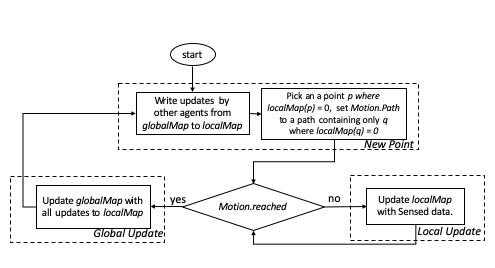
\includegraphics[width=\linewidth]{figs/map_flowchart.png}
%    \caption{Flowchart for a simple solution to 2D distributed mapping problem\vspace{-2mm}}
%    \label{fig:flowmap}
%\end{figure}
%
%
%
%We discuss now discuss how our algorithm implemented $\lgname$ shown in \reffig{mapapp} tackles $\mapprob$. \reffig{flowmap} shows a simple idea for solving this problem for each robot:
%
%The variable $\lmap$ refers to the current mapping $\map_i$ constructed by each robot $i$ using the algorithm. The function $\mathit{MaxExp}$ informally, determines whether there is a grid rectangle in the frontier of the current $\map_i$ . If not, the robot first updates its $\lmap$ from $\gmap$, which is used for sharing the currently computed occupancy maps by all agents so far. The robot then picks a new point in a rectangle known to be unoccupied in its $\lmap$ and follows a path ($\mathit{Motion.Path}$) moving only over grid rectangles known to be unoccupied by its $\lmap$. While the robot hasn't reached the target rectangle, it keeps updating its $\lmap$ with sensed data (occupied and unoccupied rectangles). When it reaches the target, it updates the $\gmap$ from its $\lmap$.
%
%
%

\subsubsection{External (Library) Functions}

% restriction of the world function for sensing. accuracy of sensor statement.
% domain of mapping function for which value is 0 or 1.
% make compatibility a definition instead of lemma.
\subsection{Assumptions}
\label{sec:formal:sensing}

The formal semantics of $\lgname$ is defined under certain timing and system information assumptions. Additionally, given that the application involves interaction with physical plants, we formally state several assumptions about low-level sensing concerns which are abstracted away by $\lgname$.

\subsubsection{Perception}


 % $\map_i(q) = 1$ indicates that according to robot $i$, there is an obstacle in $q$, $\map_i(q) = 0$ indicates that according to robot $i$, $q$ is unoccupied, and $\map_i(q) = -1$ indicates that robot $i$ doesn't have information about $q$.

%We assume that given $\Vec{x} \in q, \forall \Vec{x^\prime} \in q, \sensarea(\Vec{x}) \subseteq \sensarea(\Vec{x^\prime})$.


The sensors used by a robot for perception of the ground truth around it are \emph{Motion.trace} and \emph{Lidar.ldata}, which are \emph{sampled} sensors. Given that $\delta$ is the duration of a \emph{round},

\begin{itemize}
    \item $\mathit{Motion.trace}: [0,\delta] \mapsto \mathit{Pos}$. Given a state $\vs\in Q$ ,  $\forall i \in [N]\vs.\mathit{Motion.trace}_i = \{(t_j, p_j)\}_{j \in [M]}$ where $p_j$ is the position of the robot $i$ at time $t_j$ from the beginning of the round.
    \item  $\mathit{Lidar.ldata} : [0,\delta]\mapsto \mathit{Scan}$. Given a state $\vs\in Q$ , $\forall i \in [N], \vs.\mathit{Lidar.ldata}_i = \{t_j^\prime, l_j^\prime\}_{j^\prime \in M^\prime}$ where $l_j^\prime$ is the LIDAR \emph{scan} at time $t_j^\prime$ from the beginning of the round.
\end{itemize}

\begin{assumption}
    Given a point $p_i$, if there is a corresponding lidar scan $l_i$ when the robot is in $\qfunc(p_i)$, then there is a function $\sensfunc$ such that $\forall q\in Q$ such that $q \in \domain(\sensfunc), \sensfunc(q) = \world_Q(q)$.
\end{assumption}

$\domain(\sensfunc)$ of a robot is defined as its sensing area. This assumption is required to ensure the \emph{Individual soundess} of a mapping updated using LIDAR scan information.
\fTBD{\rg{Need to figure out how to write the assumptions so that the sensor and actuator ports don't do unexpected things during $\delta$ transitions}}
%The sampling frequencies of these sensors may be different, hence the potentially different number of readings, and potentially different timestamps of the readings.

%The function $\mathit{tSync}$ is used to \emph{synchronize} the readings, where we compute a mapping $\mathit{pScan}: \mathit{Pos} \mapsto \mathit{Scan}$, where given a state $\vs\in Q$, a robot $i\in [N]$,  $\vs.\mathit{pscan}_i = \{(p_j^{\prime\prime}, l_j^{\prime\prime})\}_{j^{\prime\prime} \in M ^{\prime\prime}}$, where  $(p, l) \in \vs.\mathit{pscan}_i$ if given $\epsilon > 0$,  $(t,p) \in \vs.\mathit{Motion.trace}, (t^\prime,l )\in \vs.\mathit{Lidar.ldata}_i, |t - t^\prime| \leq \epsilon$.

%The function $\mathit{scanToMap}: \mathit{Scan} \times \mathit{Pos}\mapsto \mathit{GridMap}$, given a position $p_i$ and its corresponding scan $l_i$, computes a quantized domain function $\sensfunc$ for .

%By definition, this returns a \emph{sound} mapping. We stated earlier that the operator $\oplus$ applied to two sound mappings returns a sound mapping. Therefore, given $s_i^\prime$ such that $\mathit{s_i^\prime \in \mathit{trans}(s_i,\mathit{LUpdate})}$,  $s_i^\prime.M.\lmap$ is sound if $s_i.M.\lmap$ is sound.


\begin{definition}
   Given a robot at a position $\Vec{x}\in D, \qfunc{\Vec{x}} = q$, the \emph{sensing area} around $q$ is a function $\sensarea: Q \mapsto 2^{Q}$ where $\forall q^\prime \in \sensarea(q), \sensfunc(q) = \world_Q(q)$.
\end{definition}

%\fTBD{define the data types in the software section}


%The function $\mathit{scanToMap}: \mathit{Scan} \times \mathit{Pos}\mapsto \mathit{GridMap}$, given a position $p_i$ and its corresponding scan $l_i$, computes the quantized domain function$\sensfunc$, in $\sensarea(\qfunc(p_i))$. By definition, this returns a \emph{sound} mapping. We stated earlier that the operator $\oplus$ applied to two sound mappings returns a sound mapping. Therefore, given $s_i^\prime$ such that $\mathit{s_i^\prime \in \mathit{trans}(s_i,\mathit{LUpdate})}$,  $s_i^\prime.M.\lmap$ is sound if $s_i.M.\lmap$ is sound.


\subsubsection{Problem Setup}

A vacuously correct (sound) solution to $\mapprob$ given $D, \qfunc$ and $\world_Q$ is $\forall i \in [N]$, $$\map_i : Q_i \mapsto \left\{0,1\right\}, Q_i = \phi$$ To allow for potentially more interesting solutions than the one stated above, we make the following assumption on the
\begin{assumption}
Initially, each robot $i\in[N]$ starts at a grid rectangle with no obstacle, the sensed area of each robot $i$ is non empty
$\forall i \in [N], \world_Q(q^0_i) = 0\wedge \sensarea(q^0_i) \neq \phi$
where $q^0_i = \qfunc(\pos_0(i))$, and $\pos_0(i)$ denotes the initial position of robot $i$.
\end{assumption}

This ensures that a robot doesn't violate the \emph{Individual soundness} requirement for a correct solution the mapping problem.

\subsubsection{Planning and actuation}

\begin{definition}
    We say that $\Vec{x_n}\in D$ is \emph{accessible} from $\Vec{x_0}$ if there is a \emph{path} $p = \Vec{x_0},\Vec{x_1}, \Vec{x_2},\ldots, \Vec{x_n}$ , such that
    \begin{itemize}
        \item $\forall i \in [0..n],\world_Q(\qfunc{\Vec{x_i}}) = 0$
        \item a robot can move from $\Vec{x_i}$ to $\Vec{x_{i+1}}$ for $i \in [0..n]$, while staying within $\qfunc(\Vec{x_i}) \cup \qfunc(\Vec{x_{i+1}})$.
    \end{itemize}
\end{definition}

A grid rectangle $q\in Q$ is accessible in general, if $\exists \Vec{x}\in D, q = \qfunc(\Vec{x})$ such that $\Vec{x}$ is accessible from either \begin{inparaenum} [(a)] \item the initial position of a robot, or \item another accessible point $\Vec{x^\prime}\in D$. We denote the accessibility of a grid rectangle using a predicate $\Access : Q \mapsto \left\{\mathit{True}, \mathit{False}\right\}$, where $\Access(q) = \mathit{True}$ if its accessible,  $\mathit{False}$ otherwise.
\end{inparaenum}

\begin{assumption}
    The path planner used by the $\lgname$ implementation of the $\dmap$ application returns a path $p = \Vec{x_0},\Vec{x_1}, \Vec{x_2},\ldots, \Vec{x_n}$ , such that the robot can traverse it while staying within $\qfunc(\Vec{x_i})$ for every $\Vec{x_i}\in p$.
\end{assumption}

This assumption can be shown to ensure for the \emph{Safe location} property of a solution, if for robot $i$, the path planner can be restricted to find paths within $\domain(\map_i)$.

%\begin{definition}
%    Given a sound occupancy mapping $\map_i$, the \emph{frontier} of $\map_i$, denoted by $\ff(\map_i)$ is defined as follows:
%    $$ \left\{ q\in Q \mid \Access(q) \wedge \exists q \in \sensarea(\Vec{x}), q \notin \domain(\map_i)\right\} $$
%\end{definition}

%Assume that the planner returns a path if \begin{inparaenum}[(a)] \item the frontier is non-empty \item the grid rectangle picked on the frontier is reachable from the current point \end{inparaenum}. We also constrain the robots to move only on \emph{known} unoccupied grid rectangles, i.e $q\in Q, s_i.M.\lmap[q] = 0$. In implementation, we achieve this by ensuring that the path planner treats all the unknown ($q$ such that $s_i.M.\lmap[q] = -1$) grid rectangles as obstacles as well.


\subsubsection{Synchronization and consistency}
The following are the timing assumptions on $\lgname$ programs.
\begin{assumption} A program step has zero logical execution time.
\end{assumption}
This assumption is reasonable if the time taken to complete a program transition step is negligible compared to $\delta$.  The $\lgname$ middleware ensures that the participating agents begin executing their events synchronously.

\begin{assumption} Shared memory updates are propagated to all agents instantanously.
\end{assumption}
The $\lgname$ middleware uses message passing to implement shared memory, and compared to $\delta$, the time taken to observe a shared memory update as a received message from the time that it is sent is much smaller. We therefore can assume that in this setting, the shared memory semantics of $\lgname$ wherein an update is visible in the next round of program transitions, is a reasonable implementation deliverable. This assumption in this particular example, is required for \emph{Eventual Completeness}, but in other applications, it may be used to correctness.
%$\marginpar{\scriptsize\sayan{MAke this a list of {\bf Assumptions} with discussion on why they hold, or what they mean in English.}}


% \rg{We can \emph{combine} the elements of the set of \emph{local maps}, $\{\map_i\}_{i\in [N]}$ to form a \emph{global} occupancy mapping. }



%
%\begin{definition}
%    Given  $i , j \in [N]$, two proposed occupancy mappings $\map_i: Q_i\mapsto\left\{0,1\right\}$ and $\map_j: Q_j\mapsto \left\{0,1\right\}$, are consistent only if $\forall q \in Q_i \cup Q_j, \map_i(q) = \map_j(q)$.
%\end{definition}




\subsection{Analysis of \dmap}
\label{sec:analysis}


In this section, we present an analysis of the $\lgname$ program for the mapping problem.
% initial states of $\A$.




Consider a state $\vs\in \Reach(\A)$. For $\vs$, the individual soundness, and the soundness requirements of the mapping problem are captured by the following invariants of $\A$ respectively.


\begin{invariant}
\label{ind-sound}
For all $i \in [N]$ $$\forall q_1 \in \domain(\vs.\lmap_i) , \vs.\lmap_i(q) =  \world_Q(q)$$
\end{invariant}

\begin{invariant}
\label{sound}
For all $i \in [N]$, $$\forall q_1 \in \domain(\vs.\gmap_i) , \vs.\gmap_i(q) =  \world_Q(q)$$
\end{invariant}

The consistency requirement of the mapping problem is captured as follows:
\begin{invariant}
\label{consistency}
For all $i,j \in [N]$, for all $q \in \domain(\vs.\lmap_i)\cup \domain(\vs.\lmap_j)$, $$\vs.\lmap_i = \vs.\lmap_j$$
\end{invariant}

We omitted the initialization of the mappings in the presentation of the program in \reffig{mapapp}. From \asum{initval}, for each robot $i$, given its initial state $\vs\in C_0$, $\vs.\lmap_i$ is a sound mapping and $\vs.\gmap_j$ is initialized to be empty, Therefore all initial states satisfy \inv{ind-sound}, and \inv{sound}.


Given $\map_i$, $\map_j$, and $q\in Q_i \cup Q_j$ , let $\map_i(q) = 1$, and $\map_j(q) = 0$. Suppose $\map_i$ is sound, then $\world_Q(q) = 1$, which implies $\map_j$ is not sound. By the same argument, if $\map_j$ is sound, $\map_i$ is not. This implies that $\vs\in C$ has individual soundness only if it also has consistency. Therefore, given $\vs\in C_0$, it satisfies \inv{consistency}.


Suppose, a state of a system $\vs\in C$ satisfies \inv{sound}, \inv{ind-sound} and \inv{consistency} , we now prove that given a transition $(\vs, a, \vs')\in \D$, $\vs'$ also satisfies them. Since these statements are only about \emph{program} variables, $\delta$-transitions don't affect them. Hence, we only need to prove that each event transition preserves these invariants.

\paragraph{NewPoint}
For every robot $i$, $\vs.\gmap_i = \vs'.\gmap_i$. Thus, this event trivially preserves \inv{sound}. So far, we haven't described the \emph{merge} function in detail, but we do so now. Given two mappings $m:Q'\mapsto \mathbb{B}$ and $n:Q''\mapsto \mathbb{B}$, the $\mathit{merge}$ function returns a mapping $\mathit{mn}: Q'\cup Q'' \mapsto \mathbb{B}$ where, \begin{itemize}
      \item for every $q \in Q'\setminus Q''$, $\mathit{mn}(q) = m(q)$
      \item for every $q \in Q''\setminus Q'$, $\mathit{mn}(q) = n(q)$
      \item for every $q \in Q \cap Q''$, $\mathit{mn}(q) = m(q) $
\end{itemize}
If $m$ and $n$ are sound, then $\mathit{merge}(m,n)$ also returns a sound mapping. Given that for every $i\in [N]$, $\vs'.\lmap_i = \mathit{merge}(\vs.\lmap_i,\vs.\gmap_i)$, and by assumption $\vs.\lmap_i$ and $\vs.\gmap_i$ are sound, $\vs'.\lmap_i$ is also sound. Therefore, this event preserves \inv{ind-sound}.

Now suppose that \inv{consistency} is not preserved, i.e. there are robots  $i, j \in [N]$, and a common $q \in \domain(\vs'.\lmap_i)\cap\domain(\vs'.\lmap_j)$, such that $\vs'.\lmap_i[q] \neq \vs'.\lmap_j[q]$. However, since $\vs'$ satisfies \inv{ind-sound}, we have proved that this event preserves \inv{consistency} by contradiction.

\paragraph{LUpdate}
Again, for every robot $i$, $\vs.\gmap_i = \vs'.\gmap_i$. Thus, this event trivially preserves \inv{sound}.

As before, we can prove as that since \emph{LUpdate} preserves \inv{ind-sound}, it also preserves \inv{consistency}.

\paragraph{GUpdate}
Since for every robot $i$, $\vs.\lmap_i$ and $\vs.\gmap_i$ are sound, by definition of \emph{merge},  $\vs'.\gmap_i$ is also sound. Therefore, this event preserves \inv{sound}. \emph{GUpdate} preserves \inv{ind-sound} trivially as it doesn't modify $\vs.\lmap_i$, and as a result, it also preserves \inv{consistency}.


%\begin{lemma}
%    \label{ext}
%    Given a robot $i$, suppose the mapping $\map_i:Q_i \mapsto \mathbb{B}$, where $Q_i\subseteq Q$, is sound. Suppose further, that the robot $i$ is is within $q'\in Q$. Consider a mapping, $\map^\prime_i: Q_i \cup \sensarea(q') \mapsto \mathbb{B}$
%    such that, $\forall q\in Q_i, map^\prime_i(q) = map_i(q)$
%    and $\forall q \in \sensarea(q'), \map^\prime_i(q) = \sensfunc(q)$. Then, $\map'_$
%\end{lemma}
%
%The proof for this is straightforward and follows from the definition of $\map^\prime_i$ combined with \defn{soundness}.
%
%Recall from the definition of the sensing area of a robot $i$ at $\pos(i)$, that it can reliably compute the ground truth mapping $\world_Q$ for all $q \in \sensarea(\pos(i))$. This lemma essentially states that given a sound occupancy mapping $\map_i$, it can be used to compute to another \emph{sound} occupancy mapping $\map^\prime_i$ by setting the values of $\map^\prime_i(\sensarea(\pos(i)))$ to the ground truth function.

%Given a mapping $\map_i$, $\domain(\map_i)$ denotes $ Q_i \subset Q$, such that $\forall q \in Q_i \map_i(q) = 0 \vee \map_i(q) = 1$.


%$Given two sound maps $\lmap$ and $\gmap$, $\lmap \oplus \gmap$ corresponds to a combined map construction as outlined in \defn{cons}, and is sound. The event \emph{NewPoint} doesn't modify $s_i.M.\lmap$ further, and therefore, $\lmap$ remains \emph{sound} during the execution of this event.

%\begin{definition}
%    We say that $\Vec{x_n}\in D$ is \emph{reachable} from $\Vec{x_0}$ if there is a \emph{path} $p = \Vec{x_0},\Vec{x_1}, \Vec{x_2},\ldots, \Vec{x_n}$ , such that
%    \begin{itemize}
%        \item $\forall i \in [0..n],\world_Q(\qfunc{\Vec{x_i}}) = 0$
%        \item a robot can move from $\Vec{x_i}$ to $\Vec{x_{i+1}}$ for $i \in [0..n]$, while staying within $\qfunc(\Vec{x_i}) \cup \qfunc(\Vec{x_{i+1}})$.
%    \end{itemize}
%\end{definition}
%
%A grid rectangle $q\in Q$ is reachable in general, if $\exists \Vec{x}\in D, q = \qfunc(\Vec{x})$ such that $\Vec{x}$ is reachable from either \begin{inparaenum} [(a)]
%                                                                                                                                                   \item the initial position of a robot, or \item another reachable point $\Vec{x^\prime}\in D$. We denote the reachability of a grid rectangle using a predicate $\mathit{Reach} : Q \mapsto \left\{\mathit{True}, \mathit{False}\right\}$, where $\mathit{Reach}(q) = \mathit{True}$ if its reachable,  $\mathit{False}$ otherwise.
%\end{inparaenum}
%
%\begin{definition}
%    Given a sound occupancy mapping $\map_i$, the \emph{frontier} of $\map_i$, denoted by $\ff(\map_i)$ is defined as follows:
%    $$ \left\{ q\in Q \mid Reach(q) \wedge \exists q \in \sensarea(\Vec{x}), q \notin \domain(\map_i)\right\} $$
%\end{definition}


\begin{theorem}
    For the system of robots $[N]$ executing the $\lgname$ program shown in \reffig{mapapp}, the shared variable $\gmap$ represents a sound mapping of the domain $Q$.
\end{theorem}

%\begin{lemma}
%    \label{ext}
%    Suppose robot $i$ is at $\pos(i)\in D$, and $\exists(q^\prime)\in \sensarea(\pos(i))$,
%    s.t $\map_i(q) = -1$. Consider a mapping, $\map^\prime_i:Q \mapsto \left\{-1,0,1\right\}$
%    such that, $\forall q\in Q \setminus \sensarea(\pos(i)), map^\prime_i(q) = map_i(q)$
%    and $\forall q \in \sensarea(\pos(i)), \map^\prime_i(q) = \world_Q(q)$.
%    Then, $\map^\prime_i(q)$ is sound if $\map_i$ is sound.
%\end{lemma}
%
%The proof for this is straightforward and follows from the definition of $\map^\prime_i$ combined with \defn{soundness}.
%
%Recall from the definition of the sensing area of a robot $i$ at $\pos(i)$, that it can reliably compute the ground truth mapping $\world_Q$ for all $q \in \sensarea(\pos(i))$. This lemma essentially states that given a sound occupancy mapping $\map_i$, it can be used to compute to another \emph{sound} occupancy mapping $\map^\prime_i$ by setting the values of $\map^\prime_i(\sensarea(\pos(i)))$ to the ground truth function.
%
%\begin{definition}
% We say that $\Vec{x_n}\in D$ is \emph{reachable} from $\Vec{x_0}$ if there is a \emph{path} $p = \Vec{x_0},\Vec{x_1}, \Vec{x_2},\ldots, \Vec{x_n}$ , such that
%\begin{itemize}
%\item $\forall i \in [0..n],\world_Q(\qfunc{\Vec{x_i}}) = 0$
%\item a robot can move from $\Vec{x_i}$ to $\Vec{x_{i+1}}$ for $i \in [0..n]$, while staying within $\qfunc(\Vec{x_i}) \cup \qfunc(\Vec{x_{i+1}})$.
%\end{itemize}
%\end{definition}
%
%A grid rectangle $q\in Q$ is reachable in general, if $\exists \Vec{x}\in D, q = \qfunc(\Vec{x})$ such that $\Vec{x}$ is reachable from either \begin{inparaenum} [(a)]\item the initial position of a robot, or \item another reachable point $\Vec{x^\prime}\in D$. We denote the reachability of a grid rectangle using a predicate $\mathit{Reach} : Q \mapsto \left\{\mathit{True}, \mathit{False}\right\}$, where $\mathit{Reach}(q) = \mathit{True}$ if its reachable,  $\mathit{False}$ otherwise.
%\end{inparaenum}
%
%\begin{definition}
%    Given a sound occupancy mapping $\map_i$, the \emph{frontier} of $\map_i$, denoted by $\ff(\map_i)$ is defined as follows:
%    $$ \left\{ q\in Q \mid Reach(q) \wedge \exists q \in \sensarea(\Vec{x}), \map_i(q) = -1\right\} $$
%\end{definition}
%
%Given a sound occupancy mapping $\map_i$, another sound mapping $\map_i^\prime$ can be constructed as shown in \lem{ext}. Taken in conjunction with our assumption on the initial positions of each robot, this leads to a strategy for computing sound occupancy mapping functions. Further, given a set of sound mappings $\left\{\map_i\right\}_{i\in[N]}$, we can construct a sound mapping $\map$ from them as follows :
%

%
%

%
%
%

% restriction of the world function for sensing. accuracy of sensor statement.
% domain of mapping function for which value is 0 or 1.
% make compatibility a definition instead of lemma.


\subsection{Implementation of Modules}

\paragraph{Sound Mapping from Synchronized Sensor Data~(ScanToMap).}
To generate a 2D map from the scan data,
it is required to synchronize the current vehicle position and the Lidar scan data.
An existing solution is to filter the time stamps of both sensor data streams
and only choose pairs of data within a given time difference threshold $\epsilon$.
This can be achieved by \texttt{ApproximateTimeSynchronizer} in the ROS package named \texttt{message\_filter}.
The frequency of the synchronized data is then limited to the sensor with the lowest frequency.
In our simulation, the lowest frequency is 100 Hz for sensing the vehicle position and sufficient for updating the map.

The Lidar scan data provided in the tool chain are pairs of a distance to obstacles and an angle with respect to the heading angle of the vehicle.
To implement ScanToMap, it is then straightforward to compute the positions of obstacles and mark occupied grid rectangles,
and to mark a rectangle obstacle free is to simply check if all four corners of a grid rectangle are covered in the scan.
The time difference $\epsilon$ however can introduce an error between real and perceived distances to obstacles.
Reducing this error is beyond the scope of this work.
Our implementation of ScanToMap therefore may falsely mark a grid rectangle as occupied when obstacles are in nearby grids.

\paragraph{Path to Frontier~(PathToFrontier).}
In the \toolname tool chain, several path planning algorithms are already available.
We particularly select the Rapidly exploring Random Tree with near neighbor search and rewiring tree~(RRT*) algorithm.
It is able to avoid obstacles and is fine tuned to the car model for simulation.
Our implementation hence only needs to choose a point in frontier grid rectangles and provide the positions of obstacles.
To choose such a point, a basic solution is to use Breadth-First Search~(BFS) on the map and seek for a unexplored grid rectangle.
BFS ensures that either all reachable grid rectangles are marked,
or there are connected unoccupied rectangles to an unexplored rectangle, and hence a path must exist.
Nonetheless, it does not guarantee that the underlying path planner can always find a path because,
for instance, the car is incapable of make sharp turns.
Our soundness claim still holds under such circumstance, but we may not be able to progress even when paths to frontier exist.
